\begin{figure*}
\centering
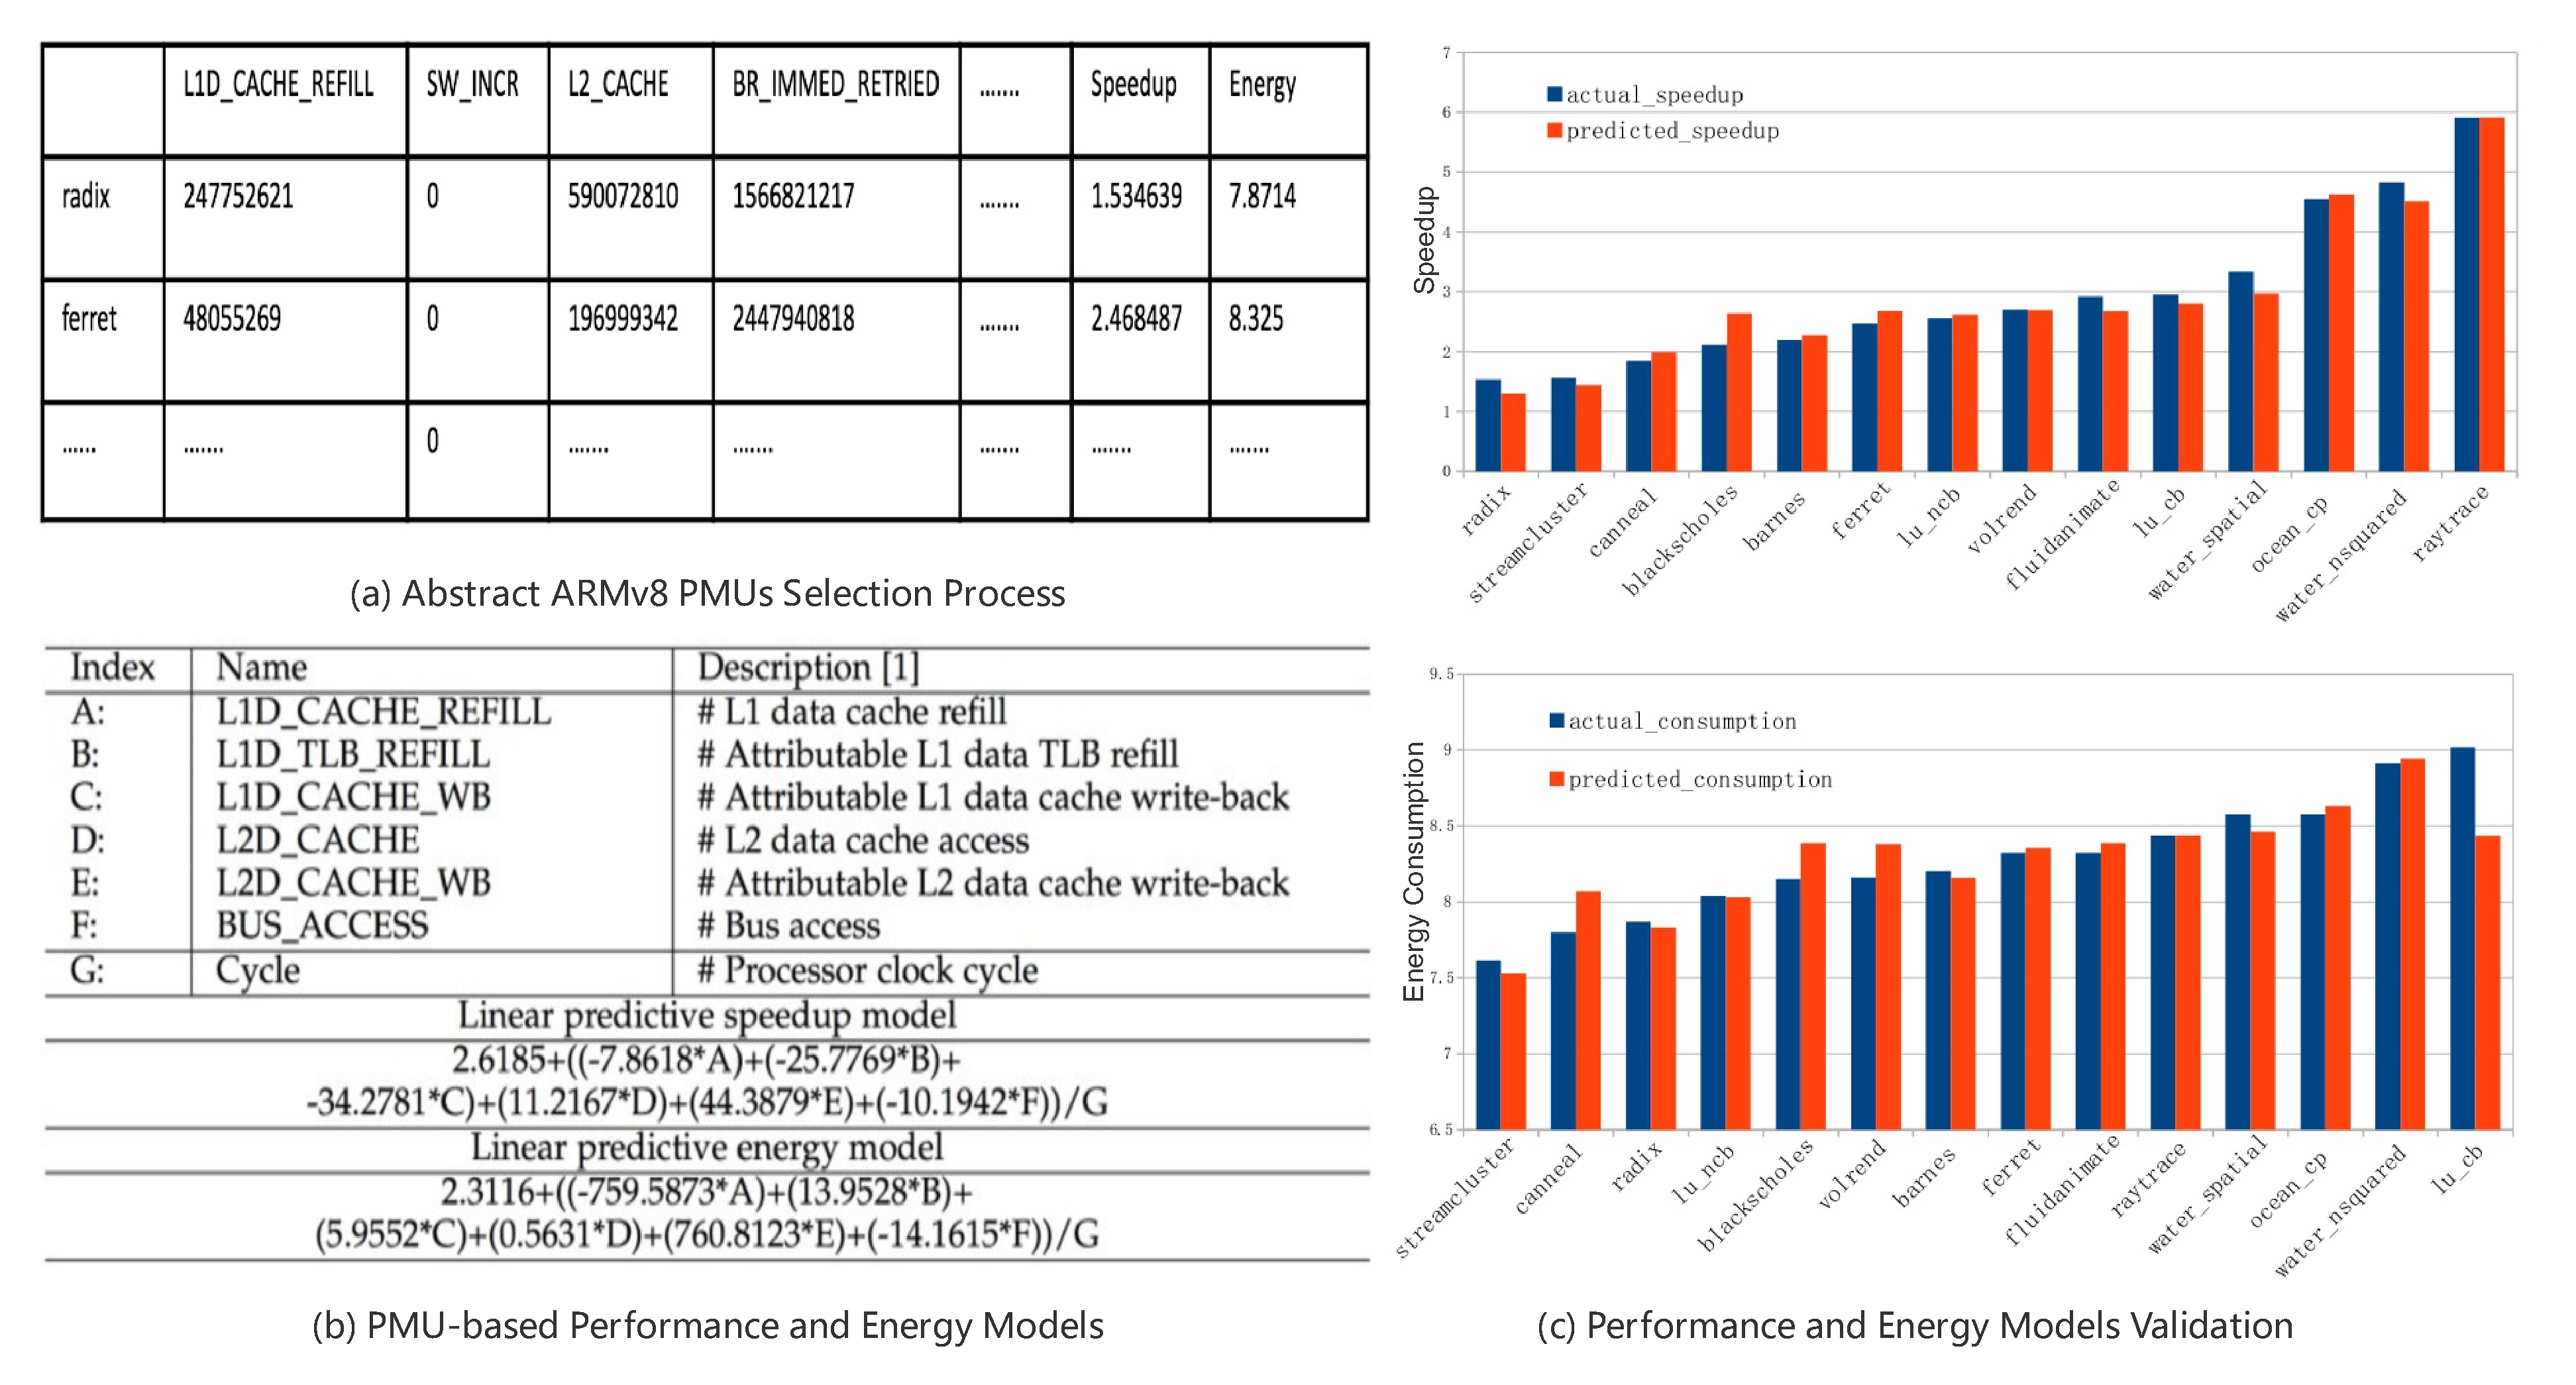
\includegraphics[scale=0.25]{figures/arm_model.pdf}
\caption{ARMv8 Performance and Energy Modelling}
\label{arm_model}
\end{figure*}

\ty{\section{Energy-Aware Scheduler Extension on ARMv8 Architecture}}

\ty{Furthermore, the energy consumption is a critical issue for multi-program co-execution on asymmetric multi-core processors. Different threads from application programs are variant between different type of cores. Followed by the prototype on GEM5 simulator, We fully-implement our COLAB scheduler on Linux kernel v3.16 with an energy-aware extension targeting ARMv8 architecture.} 

\begin{comment}
\begin{table}
  \caption{\ty{Selected ARMv8 PMUs and the Speedup and Energy Models}}
  \center
  \label{pca_arm_sp}
   \scalebox{0.8}{
   \begin{tabular}{p{0.8cm} | p{3.6cm} | p {5.4cm} c c c}
  \hline
     Index&  Name& Description \cite{ARMA57} \\
    \hline
     A: & L1D\_CACHE\_REFILL & \# L1 data cache refill\\
     B: & L1D\_TLB\_REFILL & \# Attributable L1 data TLB refill\\
     C: & L1D\_CACHE\_WB & \# Attributable L1 data cache write-back\\
     D: & L2D\_CACHE & \# L2 data cache access\\
     E: & L2D\_CACHE\_WB & \# Attributable L2 data cache write-back\\
     F: & BUS\_ACCESS & \# Bus access\\
     \hline
     G: & Cycle & \# Processor clock cycle\\
     \hline
     \multicolumn{3}{c}{Linear predictive speedup model}\\
     \hline
    \multicolumn{3}{c}{2.6185+((-7.8618*A)+(-25.7769*B)+}
    \\
    \multicolumn{3}{c}{-34.2781*C)+(11.2167*D)+(44.3879*E)+(-10.1942*F))/G}\\
 \hline
  \multicolumn{3}{c}{Linear predictive energy model}\\
     \hline
    \multicolumn{3}{c}{2.3116+((-759.5873*A)+(13.9528*B)+}
    \\
    \multicolumn{3}{c}{(5.9552*C)+(0.5631*D)+(760.8123*E)+(-14.1615*F))/G}\\
 \hline
  \end{tabular}}
\end{table}
\end{comment}

\ty{\subsection{Machine Learning based ARMv8 Performance and Energy Models}}

\ty{The abstract offline PMU selection process is shown in Fig.~\ref{arm_model}(a). We first run all benchmarks compiled in single-threaded version on either 4 Cortex-A73 or 4 Cortex-A53 configuration. We only record common PMUs used for both Cortex-A73 and Cortex-A53, together with each thread's relative speedup and energy consumption. We ignore the PMUs for which their value keep to be zero, such as \texttt{SW\_INCR} (Instruction architecturally executed, Condition code
check pass, software increment). For the remaining PMUs, we then apply the PCA technique to select the most important 6-PMU-combination. For example, it is easy to know that the performance and energy will be more dominated by the total data movement than some branch behaviours. As a result, although \texttt{BR\_IMMED\_RETIRED} is a meaningful PMU which counts all immediate branch instructions that are architecturally executed, but it is not selected after the PCA process as there are more important PMUs such as \texttt{L1D\_CACHE\_REFILL} (L1 data cache refill) and \texttt{L2\_CACHE} (L2 data cache access). }

\ty{The trained PMU-based ARMv8 performance and energy models are shown in Table~\ref{arm_model}(b).
In real ARM system validation, we use the clock cycle number to replace the GEM5 committed instructions as it is more stable recorded by a specialized register on the test board.}

\ty{We validate the accuracy of our trained models on each benchmark as shown in Fig.~\ref{arm_model}(c). The average error cross all benchmark for the performance model is around 7\% while for the energy model is around 1.5\%.}
%The range of these errors are within the normal performance and energy variance of the test board, so we can claim that the trained models are accuracy enough to predicate the system behaviours.}

\ty{\subsection{COLAB Algorithm Extension}}

\begin{algorithm}
\caption{Energy-aware COLAB extension}
\label{alg:2}
\begin{algorithmic}[]
\STATE \textbf{\_core\_alloctor\_e(thread\_struct\ $t$)}\{
\STATE \textbf{if} t.high\_hyper
\STATE \ \ \textbf{return} rr\_allocator\_(big\_cores)
\STATE \textbf{if} {t.low\_hyper \& t.low\_block}
\STATE \ \ \textbf{return} rr\_allocator\_(little\_cores)
\STATE \textbf{else return} rr\_allocator\_(cores) \}
\end{algorithmic}
\end{algorithm}

\ty{The original COLAB scheduler is extended to involve further collaboration to achieve energy-aware extension. Under this extension, a hyper-heuristic of a thread $t$ to guide core allocation is designed as follows:}
\ty{$$ hyper\_(t) = w_{s}*speedup(t) + w_{e}*energy(t) $$}
\ty{Where $w_{s}$ and $w_{e}$ are the trained weights of the speedup factor and energy consumption factor, separately; $energy(t)$ is the energy efficient factor for the thread $t$ between big and little cores. Energy efficient is the ratio of useful work done to the amount of power used as introduced in~\cite{tsirogiannis2010analyzing}. Similar with using linear regression on training PMUs for predicated speedup and energy consumption, this hyper-heuristic is trained by hierarchical regression to obtain the best trade-off between performance gain and energy saving.}

\ty{The extended energy-efficient core allocator \texttt{rr\_allocator\_e()} for the COLAB scheduling algorithm is presented in Alg.~\ref{alg:2}. Compared with the original version, it uses this hyper-heuristic to replace the speedup-heuristic in \texttt{rr\_allocator\_()}. Similar with mapping high speedup threads on big cores, this trade-off allocation policy is applied to avoid heavy energy consumption on big cores. When the energy-aware extension is enabled, threads labeled by this hyper-heuristic involve both the performance and energy concerns instead of the predicated speedup only. Under this hyper-heuristic, core allocator can provide the energy-aware solutions. It only allocates high speedup and non-energy-intensive threads to big cores, while keeps energy-intensive threads on little cores even they also have some kind of speedup.} 

\ty{\subsection{Scheduling Overhead Analysis}}
The overhead of the performance model is small. It is updated only every 10 msec and it requires the evaluation of the linear regression equation for each thread. 

\ty{To maintain per task runtime counter information, we need to access the hardware PMUs every time we context switch. By using register to read a PMU directly, it takes 4 cycles on the Cortex-A53 and 14 cycles on the Cortex-A73. We need to read 7 PMUs in sequential each time.}

The rest of scheduling overhead comes from labeling all threads based on predicted speedup and blocking level every 10 msec. This is similar to the scheduling overhead of WASH and is infrequent enough to not affect us.

